\documentclass{article}

% if you need to pass options to natbib, use, e.g.:
% \PassOptionsToPackage{numbers, compress}{natbib}
% before loading nips_2016
%
% to avoid loading the natbib package, add option nonatbib:
% \usepackage[nonatbib]{nips_2016}

\usepackage[final, nonatbib]{nips_2016}

% to compile a camera-ready version, add the [final] option, e.g.:
% \usepackage[final]{nips_2016}

\usepackage[utf8]{inputenc} % allow utf-8 input
\usepackage[T1]{fontenc}    % use 8-bit T1 fonts
\usepackage{hyperref}       % hyperlinks
\usepackage{url}            % simple URL typesetting
\usepackage{booktabs}       % professional-quality tables
\usepackage{amsfonts, amssymb, amsmath}       % blackboard math symbols
\usepackage{nicefrac}       % compact symbols for 1/2, etc.
\usepackage{microtype}      % microtypography
\usepackage{graphicx}
\usepackage{algpseudocode}
\usepackage{algorithmicx}


\graphicspath{ {images/} }

\title{Hidden warnings; using topic modeling on Yelp reviews to predict health inspection violations}

% The \author macro works with any number of authors. There are two
% commands used to separate the names and addresses of multiple
% authors: \And and \AND.
%
% Using \And between authors leaves it to LaTeX to determine where to
% break the lines. Using \AND forces a line break at that point. So,
% if LaTeX puts 3 of 4 authors names on the first line, and the last
% on the second line, try using \AND instead of \And before the third
% author name.

\author{
  Michael Bostwick\\
  Department of Statistics and Operations Research\\
  University of North Carolina at Chapel Hill\\
  \texttt{mgb2188@live.unc.edu} \\
}

\begin{document}
% \nipsfinalcopy is no longer used

\maketitle
\begin{abstract}
  This paper offers an approach for using social media data to make public policy decisions through the application of 
  predictive and interpretable topic models. Most applications of machine learning benefit from interpretability, but 
  particularly those proposed to be used in the public domain. Within the realm of topics models, prior work has found 
  supervised Latent Dirichlet Allocation (sLDA) to surpass unsupervised Latent Dirichlet Allocation (LDA) 
  in predictive power, while still remaining interpretable to human users.  We test sLDA and a simple historical model on a 
  dataset of Yelp text reviews associated with restaurant health inspection scores. Findings suggest sLDA effectively 
  discovers an overall document structure, but struggles to extract a strong predictive signal on this dataset.
\end{abstract}

\section{Introduction}
Local governments have limited resources to carry out monitoring and inspection of restaurants, yet the CDC estimates that 48 
million people get sick from foodborne illnesses in the United States each year \cite{cdc}. In recent years there 
has been increased interest for local governments to not only release more of their own open data, but to 
repurpose other data to improve efficiency and effectiveness \cite{glaeser}. A prime source of data relating to restaurants can
be found on Yelp, a review crowdsourcing platform for all types of businesses, but most popular for food and beverage 
establishments. On Yelp customers can leave numeric ratings (on a scale of 1-5) and text reviews of a particular business they
have visited. In larger metroplitan areas it is common for a restaurant to have hundreds or thousands of reviews, providing 
lots of potential clues to the hygiene of a restaurant. This Yelp data can then be linked to publicly available city health inspections scores in the hopes of optimizing inspection operations. If city officials could predict which restaurants are most likely to be violating the health code, inspection resources could be reallocated for a combination of cost savings and increased food safety. Currently, it is common for cities to carry out their inspections randomly and uniformly.

While there is a large amount of metadata associated with Yelp reviews (time of review, average rating of reviewer, etc.), 
this work will focus on just the text review itself. In order to peform regression or classification from text, it is typical 
to transform the text into a bag-of-words, that is each unique word is a feature and cell values represent its occurence, 
disregarding word order. From there standard machine learning algorithms can be applied to the dataset, but since there are 
many unique words in the english language the dimensionality is usually very high. This dimensionality challenge, both for 
predictive power and interpretability will be examined in further detail 
throughout the paper.

This paper is organized as follows. We first review two streams of related work, those pertaining to the application of social
media to civic functions and those pertaining to the techniques used in topic modeling. Next, we elaborate on the model and 
how inference and learning can be performed on it. From there we evaluate the procedure on synthetic data and a combined Yelp 
and health inspection dataset from Seattle, WA, comparing several approaches. Lastly, we discuss considerations that 
make this approach more or less favorable.

\section{Related Work}

\subsection{Applications}

This paper primarily builds off of similar work by Kang et al. \cite{kang} who predicted health inspection scores from Yelp
data for Seattle restaurants. Their work included many aspects of the review and restaurant data, including zip code and 
inspection history and unigram + bigram text features, which were then input to a Support Vector Machine (SVM). They formulated their prediction task as a classification problem and only considered restaurants with zero violations, "hygienic", or many 
violations, "unhygienic". As Kang et al. found the text review contents to generate the most promising features, we focus the 
experiements in this work just on them. Joaristi et al. \cite{joaristi} also build on this work, but with a differing approach
. They apply Latent Dirichlet Allocation (LDA) to extract topics separately from the positive and negative text reviews and 
then use these topic features along with other generated features as inputs into SVM, logistic regression and Random Forest 
algorithms.

\subsection{Topic Modeling}

Topic modeling is a well established \cite{blei} technique to reduce the dimensionality of a set of text documents, 
typically in an unsupervised fashion. This can be very helpful for tasks like browsing documents or determining document 
similarity, but may not build the best features for prediction tasks. This paper focuses on one technique to address this 
concern, supervised Latent Dirichlet Allocation (sLDA) \cite{mcauliffe}. sLDA allows a set of topics to be modeled on documents with the addition of a response variable. The promise is that sLDA not only discovers a latent structure of documents, but one that explains the response 
variable.There have been other efforts to guide LDA topic models, one such work done by Jagarlamudi et al. \cite{jagarlamudi} 
in which the user can provide a set of seed words to encourage a set of topics. Such an approach is not tested here, but 
offers an interesting technique to explore with further experiments.

\section{Model}

\begin{figure}[h]
\centering
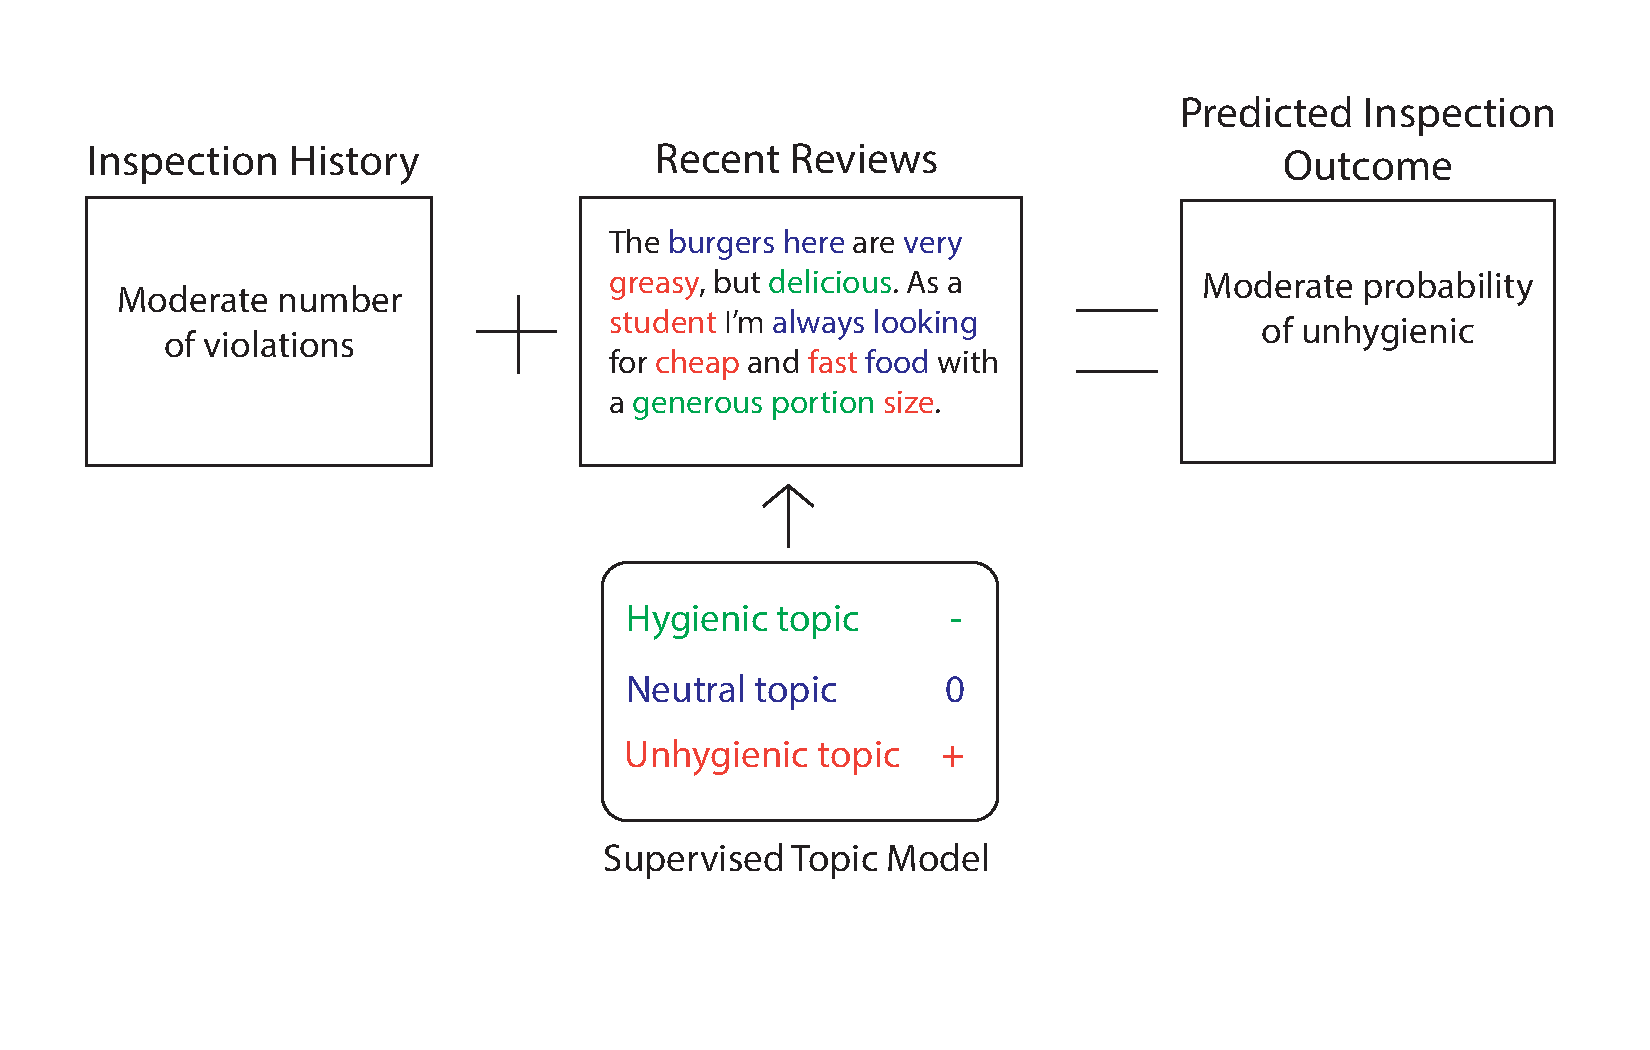
\includegraphics[scale = 0.5]{figure1}
\caption{In the hypothetical example above the restaurant's inspection history does not provide a clear prediction so we need 
to make use of recent review text. In the review there are 5 words from the unhygienic topic and only 3 words from the 
hygienic topic, so we would predict the restaurant to be unhygienic, but not overwhelmingly so.}
\end{figure}

\subsection{Overall model}
At a high level the overall model is illustrated in Figure 1. For each restaurant we take information about their 
previous inspection history and then combine that with information extracted from topic modeling of recent reviews. The 
assumption is that predictions for historically very hygienic or very unhygienic restaurants can be made fairly easily and for
restaurants in the middle, recent customer feedback can hint at a problem or not. For the inspection history we build a simple
logistic regression model including the average number of health violations and the number of health violations on the
previous inspection. Finding the previous number of violations to not be a significant factor, we limit the model to just
use the average number of violations. We discuss the process to extract information from text reviews in the next section, 
but once obtained we then combine the two preliminary models using a decision tree and then use the combined decision tree 
model to produce the final prediction.

\subsection{Supervised Latent Dirichlet Allocation}

\begin{table}[h]
\begin{center}
\begin{tabular}{l l l l }
$\theta$ & Topic proportions & $\beta$ & Term proportions \\
$\alpha$ & Prior on topic proportions & $y$ & Response variable \\
$z_{n}$ & Topic assignment & $\eta$ & Topic coefficients \\
$w_{n}$ & Word & $\sigma^{2}$ & Variance of response variable\\
$K$ & Number of topics & $N$ & Number of words \\
\end{tabular}
\end{center}
\label{notation}
\caption{Notation}
\end{table}



The intuition behind LDA is that within a collection of documents, each is made up of a mixure of latent topics. This a
relaxation of classical mixture models, each document is not restricted to one topic. Each document has a unique mixture 
proportion drawn from a dirichlet distribution. The latent topics are observed in the data through words, where each topic is 
a unknown distribution of words over the vocabulary. A response variable is added in sLDA that is then jointly modeled with 
the documents \cite{mcauliffe}.

Formally, each document and response is generated from the sLDA model as follows: \newline
1. Draw topic proportions $\theta | \alpha$ $\sim$ Dir($\alpha$) \newline
2. For each word \newline
  (a) Draw topic assignment $z_{n} | \theta \sim$ Mult($\theta$) \newline
  (b) Draw word $w_{n} | z_{n}, \beta_{1:K} \sim $ Mult($\beta_{z_{n}}$) \newline
3. Draw response variable y $| z_{1:N}, \eta, \sigma^{2} \sim$ N($\eta^{T}\bar{z},\sigma^{2}$) \newline
Where $\bar{z}$ is defined as $\frac{1}{N} \sum_{n=1}^{N} z_{n}$.

\begin{figure}[h]
\centering
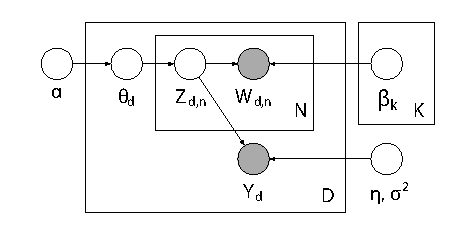
\includegraphics[scale = 1]{slda_graphic}
\caption{A graphical model representation of sLDA from \cite{mcauliffe}}
\label{fig_slda}
\end{figure}


\subsection{Inference and Learning}
Inference and learning for the model is carried out through Monte Carlo EM as implemented in the LDA package in R \cite{changR}. 
This is in contrast to the variational EM procedure outlined in \cite{mcauliffe}. For the E step a collapsed Gibbs sampler is
used to compute $\mathbb{E}[\bar{z}]$ and then standard regression (logistic in this case) is carried out for the M step. The 
collapsed terminology refers to the integrating out of $\theta$ (the document distributions over topics) and $\beta_{k}$ (the 
topic distributions over words), so that we are left with the topic assignments for each word, $z_n$. To sample from the 
posterior we compute the posterior for a single assigment conditioned on all other assignments. For sLDA the posterior can be 
found to be Equation \ref{eq:posterior} as derived in \cite{chang}. The terms after the $\propto$ on the first line are the same as used in LDA and the terms on the second line are the part needed for also modeling the response variable.

\begin{align}
 p(z_{d,n} = k|\alpha,\eta,\textbf{w},\textbf{y},\textbf{b},a,\mathbf{z_{-(d,n)}}) \propto & (n^{\neg d,n}_{d,k} + \alpha_{k})
 \frac{n^{\neg d,n}_{w_{d,n},k} + \eta_{w_{d,n}}}{N^{\neg d,n}_{k} + W\eta}\cdot \nonumber \\
  & exp(2\frac{b_{k}}{N_{d}}(y_{d}-a-\mathbf{b}^{T}\mathbf{\bar{z}}^{\neg n}_{d} - (\frac{b_{k}}{N_{d}})^{2})  \label{eq:posterior}
\end{align}

When computing the posterior we exclude the topic assignment for the current word so $n^{\neg d,n}_{d,k}$ is the number of 
words assigned to topic $k$ in document $d$ excluding the current assignment, $n^{\neg d,n}_{w_{d,n},k}$ is the number of 
times word $w$ has been assigned to topic $k$ excluding the current assignment and $N^{\neg d,n}_{k}$ is the number of times 
topic $k$ has been assigned excluding the current assignment. We can see that the probability of $z_{d,n}$ is a combination of how often topic $k$ occurs in document $d$, how often word $w$ occurs in topic $k$ and how well topic $k$ helps predict the response variable $y_{d}$.

$\textbf{Algorithm 1}$

\begin{algorithmic}[1]
\State $z \gets random\ initialization$
\For{$m\gets 1, M$} \Comment{M-step iterations}
  \For{$e\gets 1, E$} \Comment{E-step iterations}
      \For{$d\gets 1, D$} \Comment{Documents in corpus}
        \For{$n\gets 1, N$} \Comment{Words in document}
          \State $z_{d,n} \gets \max_{k} p(z_{d,n} = k)$ \Comment{From Equation \ref{eq:posterior}}
        \EndFor
      \EndFor
   \EndFor
   \State $fit \gets regression(\bar{z},\eta,\sigma^{2})$
\EndFor
\end{algorithmic}


The complete sLDA procedure can be seen in Algorithm 1. For prediction on the test data, we perform inference just using the 
LDA portion of Equation \ref{eq:posterior} to determine $\bar{z}$ and then predict using the fitted logistic regression model.

\section{Data}
\subsection{Description}
For our experiments we use the benchmark dataset from Kang et al. \footnote{Data is available at: http://www3.cs.stonybrook.edu
/~junkang/hygiene/}. There are about 13,000 observations, each corresponding to an inspection, from about 152,000 reviews made
at over 1,756 restaurants in the Seattle, WA area. Reviews are matched to inspections if they fall on or before the inspection date, but after the previous inspection date. In order to filter out possible fake or deceptive reviews, Kang et al. have 
removed reviews that are at least 2 stars away from the restaurant's average star rating on Yelp. The violation scores found 
in the dataset range from zero to 115, with a median of 7 and mean of 12.18. 

Since restaurants with severe violations are of most interest, we 
transform this to a classification problem by definining inspections with violations above a threshold $\tau$ as "unhygienic" 
and inspections with zero violations as "hygienic", as also done by Kang et al. We remove inspections that fall in the middle 
for two reasons, to keep relative class balance and because there is little signal in the reviews of these inspections. Prior 
intuition and review of the data shows that reviewers may comment on hygiene if it is particularly bad or particularly 
good, but neutral opinions are oftern left unsaid. We set $\tau = 20$ as it is a large enough threshold to distinguish 
the two classes, but not so large as to severely imbalance the classes. This leaves 7,930 observations, which we split 50/25/25 into training, validation and test sets, respectively. Below are three examples of review text. In the first two examples 
there are clear suggestions of an unhygienic restaurant in the text, but only the first example had any violations. On the 
other hand, in the third example there is no discussion of hygiene at all, but the inspection found a violation score of 43.

\subsection{Example data}
\small
Easy (Violation Score = 40): "...Next thing I ordered was the Bok Choy Pork Buns, about to pick up the last one to eat and find a 
FRIGGIN BABY COCKROACH. Now I  have my safe serve license from New York its a lot more in depth than Washington. An Adult 
cockroach is just kinda a roamer but a baby means TOTAL INFESTATION. Its friggin disgusting! They didn't charge me for the 
dish but should have comped me for the meal. I left right then and there. How can you serve a ROACH on a platter? I wouldn't 
recommend going there at all if you are not concerned about your health..." \newline

Hard (Violation Score = 0): "OMG!These guys need to use some bleach in this place. I enjoy a good dive once in a while but this place
has been on the down slide for many years now. How they stay open I have no idea.Many moons ago, this place served up some 
pretty decent dim sum, now it borders on a health code violation...." \newline

Hard (Violation Score = 43): "Imagine sitting on a tropical island slurping down drinks; the ones made with various rums, little 
umbrellas and fresh fruit garnishes. Bamboo serves all kinds of these and they're fairly potent as well. They have a large 
menu with good sized portions and the prices are right. The service is usually pretty good, but it might suck too. It just 
depends on the day. The best seats are on the sidewalk in the "bamboo corral" and it doesn't get any better than on a sunny 
day. The inside decor kind of creeps me out, so I like to sit as close to the window as possible to look out at Alki. All in 
all, a great place to go when it's hot and sunny, or even when it's not..." \newline

\normalsize

\subsection{Vocabulary pre-processing}
When fitting the sLDA model all unique words can be used, but it is common practice to filter down to a more computationall 
manageable and informative vocabulary. After performing standard text pre-processing (making all characters lowercase and 
removing punctuation, numbers and stop words) we evaluate the term frequency-inverse document frequency (Equation 2) for each term and keep the top 4,000 terms (out of 10,912). We then take this 4,000 term vocabulary and build a 
sparse document term matrix, each row represents the reviews for an inspection, each column is a term and the cell values are 
the number of occurrences.

\begin{equation}
tfidf = mean(\frac{f_{t}}{|d|})*log(\frac{|D|}{n_{t}}) \label{eq:tfidf}
\end{equation}
Where$\colon$ \newline
$f_{t}$ = frequency of term $t$ in document $d$ \newline
$D$ = corpus of documents \newline
$n_{t}$ = number of documents that term $t$ appears in \newline

\section{Evaluation}

\subsection{Synthetic data}
To test the sLDA procdedure we create a synthetic dataset following the generative process described in Section 3.2. That is, 
first we fix the model parameters to K = 3, $\alpha = 1$, $\beta_{k} \sim Dir(0.1)$, $\eta^{T} = (1, 15, 25)$ and $\sigma^{2} 
= 2$. Then we generate 100 documents of 20 words each with accompanying response variable y, drawn from  $N(\eta^{T}\bar{z}
,\sigma^{2})$. While we use class response labels for the real data, for simplicity here we consider the case y $\in \mathbb{R
}$. After fitting the sLDA model we get the output seen in Table 2 and a prediction RMSE of 2.2, a 
reasonable result given the variance of 2 for the Normal distribution that we draw the response variable from. In addition to 
prediction, it can be seen that for the most part the sLDA procedure has accurately recovered the word distributions for
each topic.

\begin{table}[h]
\begin{center}
\begin{tabular}{l l l l | l l l l}
\multicolumn{4}{c |}{Generative} & \multicolumn{4}{c}{Inference}\\
\hline
 & Topic 1   & Topic 2 & Topic 3 & & Topic 1   & Topic 2 & Topic 3 \\
\hline
$\eta$ & 1 & 15 & 25 & $\hat{\eta}$ & 2.03 & 14.1 & 25.43 \\
 & word15 & word4 & word1 & & word15 & word4 & word1 \\
 & word6 & word17 & word2 & & word6 & word17 & word2\\
 & word4 & word1 & word14 & & word20 & word19 & word14\\
 & word20 & word15 & word12 & & word4 & word1 & word12 \\
 & word3 & word19 & word17 & & word1 & word10 & word5\\
 \\
\end{tabular}
\end{center}
\label{synthetic}
\caption{Topic coefficients and top 5 words for generated data and results of sLDA inference. The sLDA process has effectively recovered both the topic coefficients and word distributions.}
\end{table}

\subsection{Yelp and Health Inspection data from Seattle}
We train sLDA on the Seattle data using 10 topics, setting $\alpha = 50/k$ and $\beta_{k} \sim Dir(0.1)$ as suggested in 
\cite{griffiths}, and running for 50 iterations of the EM with 20 passes of collapsed gibbs sampling for each iteration. 
Running for additional iterations yielded little improvement in the validation accuracy. Also, when fitting an LDA model to 
this data the change in log likelihood levels off by 50 iterations. 

We can see a representation of the topics found through sLDA on the real data in Figure \ref{fig_topics}. The topics discovered are easily interpretable as they closely fit to different types of cuisine. As most restaurants serve a single type of 
cuisine this matches the document structure. The sLDA model has found that restaurants represented by topics to the right are 
more likely to be unhygienic than topics to the left. Unfortunately for the predictive aims here, this is not the most helpful
topic structure as it shows little temporal information about a restaurant. For example, chinese restaurants will always have 
review text dominated by the furthest right topic and an uptick in unsanitary practices noted by reviewers will not be 
discovered.

\begin{figure}[h!]
\centering
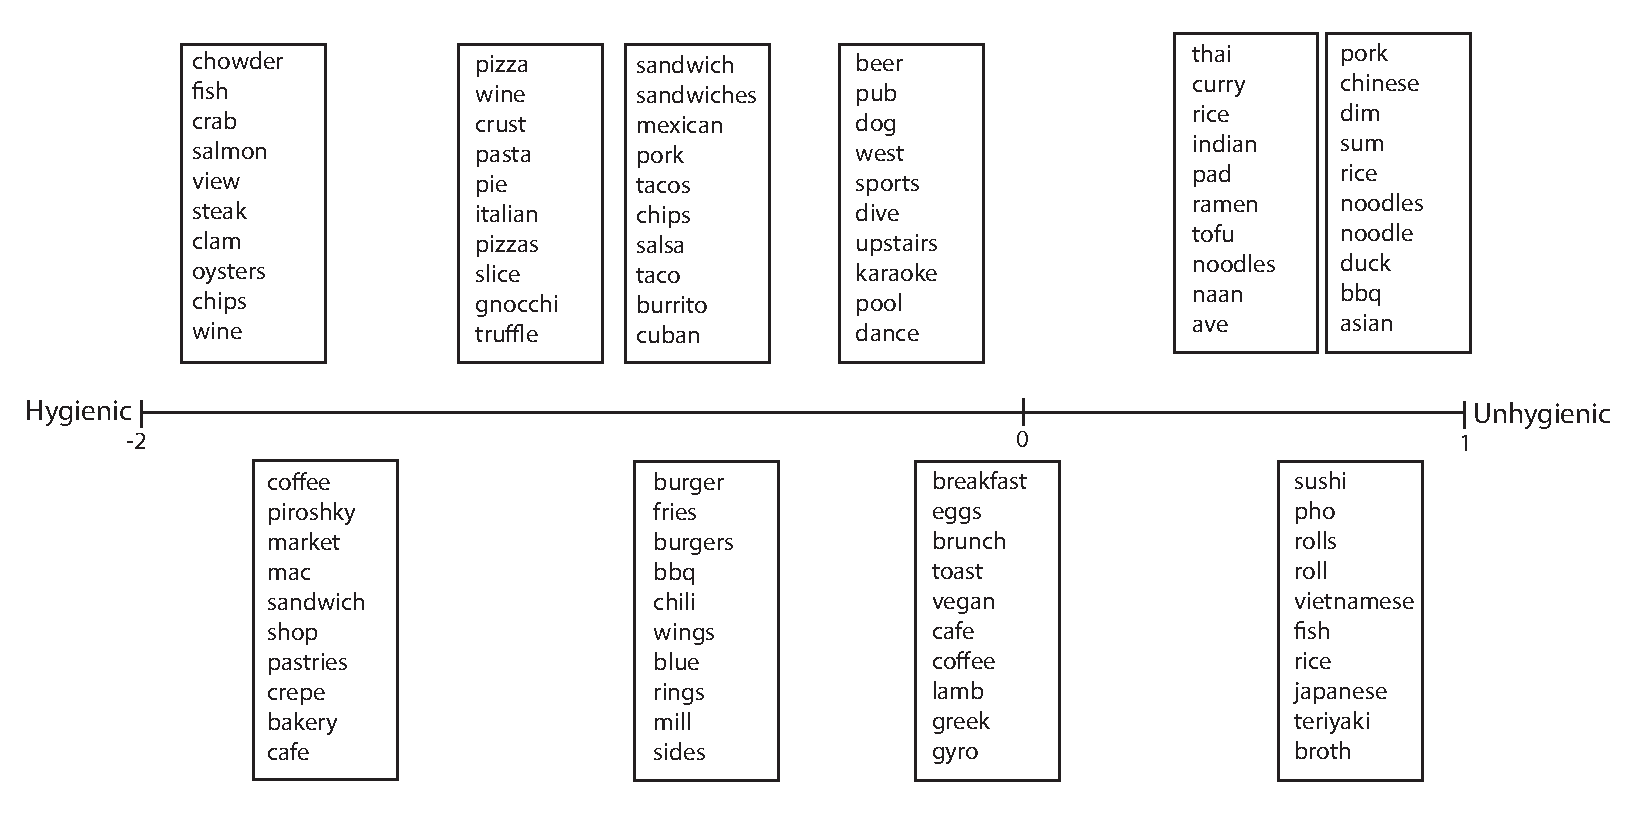
\includegraphics[scale = 0.5]{topics}
\caption{Top ten words from topics found through sLDA. Topics are organized horizontally according to their logistic regression coefficient, with the "unhygienic" class being positive.}
\label{fig_topics}
\end{figure}

The results of combining the history model and the sLDA model through a decision tree can be seen in Figure \ref{tree}. This 
tree is easily interpretable and makes intuitive sense. For restaurants with a low historical average of violations we predict
"hygienic" and for those with a high historical average of violations we predict "unhygienic". For those in the middle we
consult the sLDA model and if the probality of unhygienic is above 0.48 we predict "unhygienic".

A comparison of the history model, sLDA model and combined model can be seen in Table 3 and Figure \ref{ROC}. The 
history model and sLDA perform similarly, but the history model has the advantage in both accuracy and Area under the curve 
(AUC). The combined model has a slightly higher accuracy than the history model, but the receiver operating character (ROC) 
curve shows little difference between the two.  

\begin{table}[h]
\begin{center}
\begin{tabular}{l l l}
Method   & Accuracy & AUC \\
\hline
History  & 0.649 & 0.676 \\
sLDA     & 0.628 & 0.639 \\
Combined & 0.656 & 0.673 \\
\end{tabular}
\end{center}
\label{results}
\caption{Results}
\end{table}

\begin{figure}[h!]
\centering
\begin{minipage}{.5\textwidth}
  \centering
  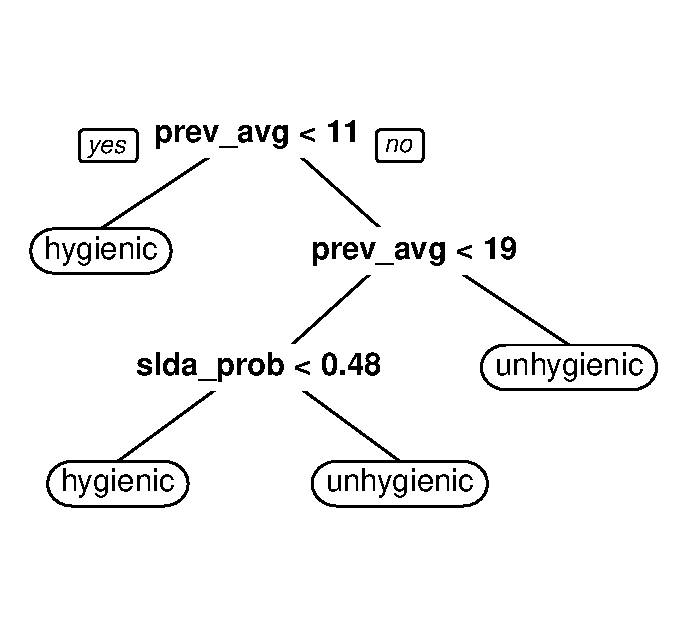
\includegraphics[width=.8\linewidth]{decision_tree}
  \caption{}{Combined model decision tree}
  \label{tree}
\end{minipage}%
\begin{minipage}{.5\textwidth}
  \centering
  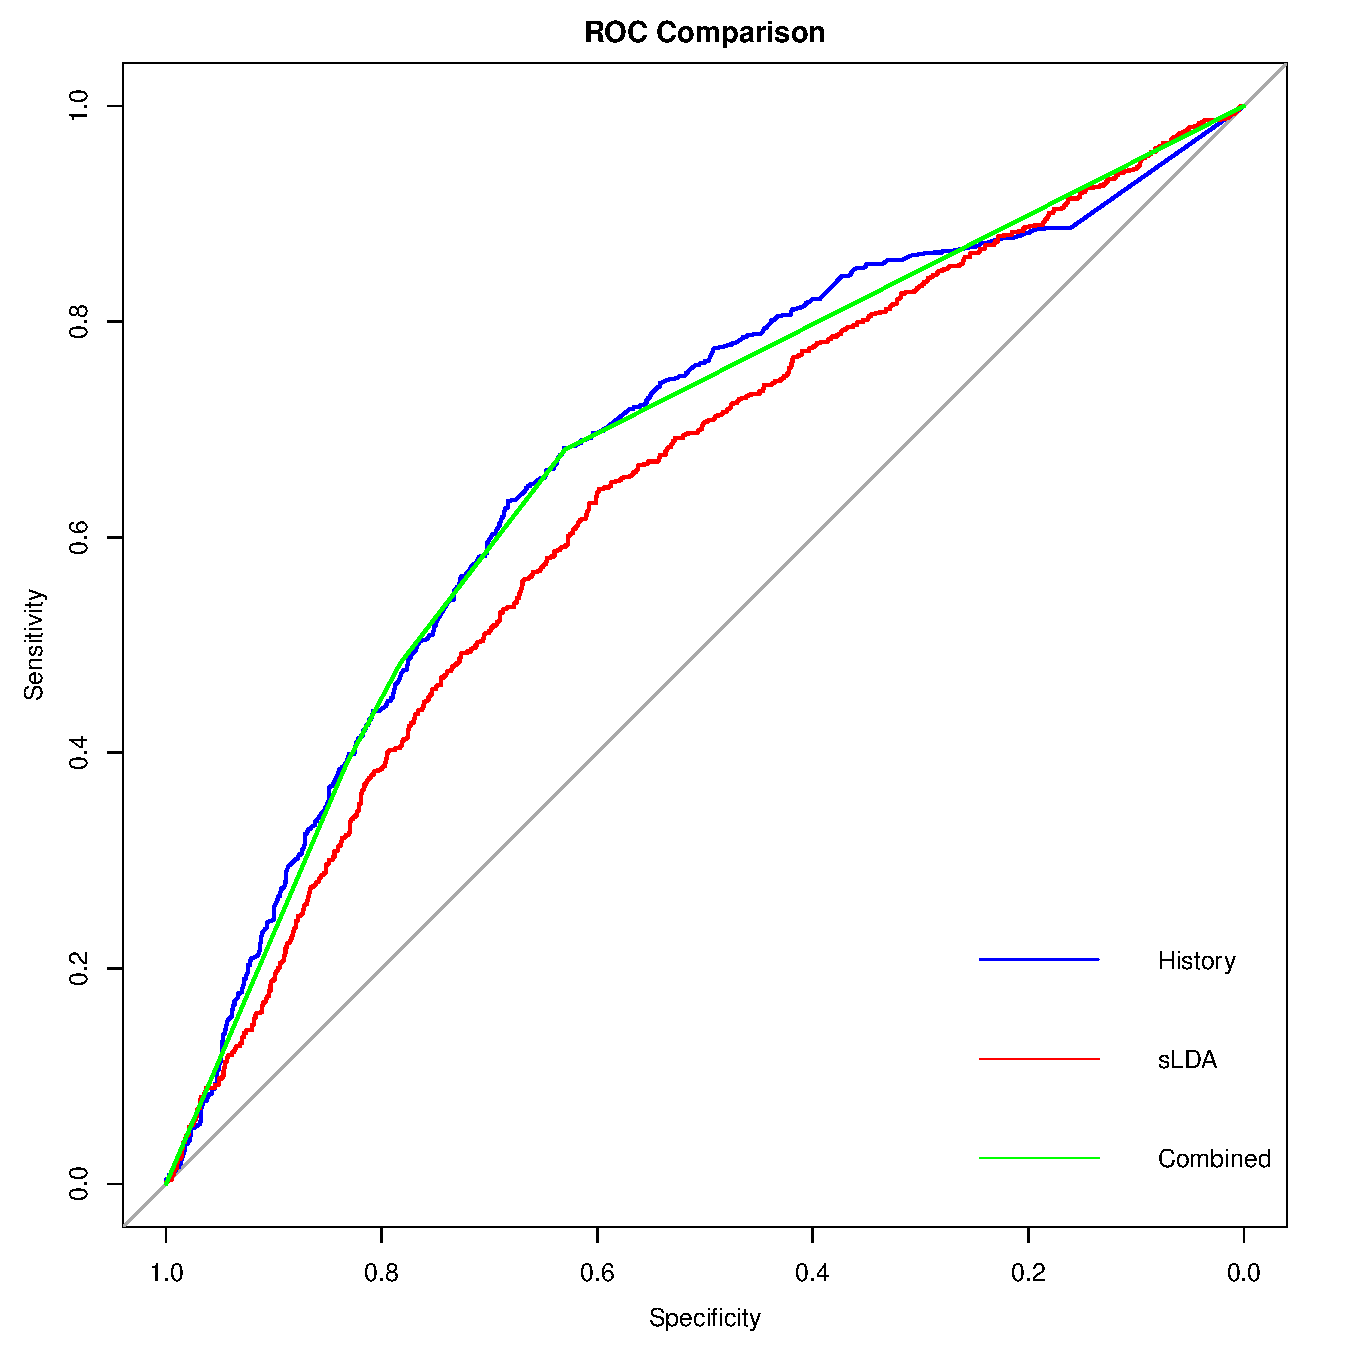
\includegraphics[width=.8\linewidth]{roc_compare}
  \caption{}{ROC Comparison}
  \label{ROC}
\end{minipage}
\end{figure}



\section{Discussion}

\subsection{Model comparison}
Since the sLDA model was found to have interpretable, but not highly accurate results we look into possible reasons why. A 
plot of the predicted probability of the history model and sLDA model can be seen in Figure \ref{correlation}. The lack of any clear trend in this plot suggests that even though the two models have similar accuracy there is not a strong correlation between their predictions. If there was a strong correlation visible in this plot the small improvement in the combined model would be expected as the two preliminary models would be providing duplicative information.

\begin{figure}[h!]
\centering
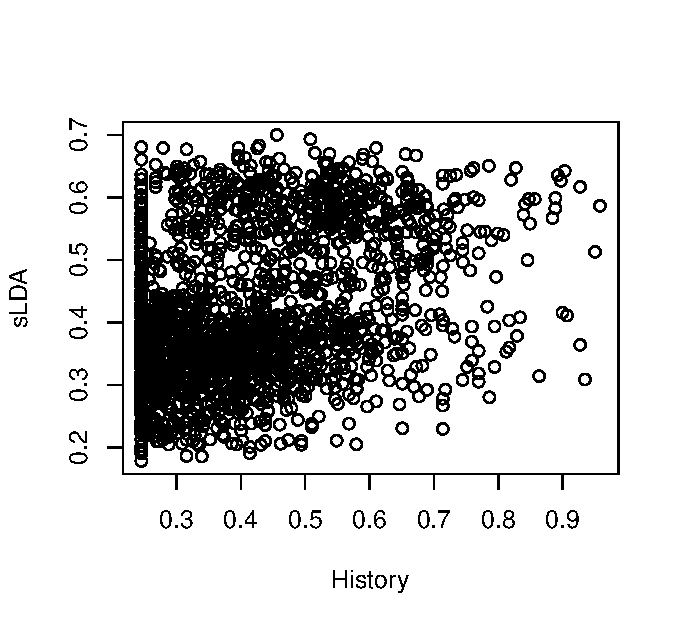
\includegraphics[scale = 0.75]{prediction_correlation}
\caption{Plot of predicted probability of unhygienic for each model}
\label{correlation}
\end{figure}

\subsection{Word analysis}
By examining what topics are assigned to particular words we can gain a better understanding of the underlying model. For example, the suggestively unhygienic word "roach" appears 19 times in the almost 4000 training documents and the sLDA model assigns it to the "Chinese" topic half the time and the "Thai" topic all but one of the remaining times. Not all of these 19 training documents are restaurants serving Chinese and Thai cuisine, but the majority are. In addition, the words most associated with "roach" are "roaches", "cockroach", "crawling", "dimsum", "jade", "gao", "garden", "dim", "sum", "richmond". So while a human would likely consider "roach" to be a part of a separate unhygienic topic, because of the strong co-occurrence with particular cuisine words the topic model is not able to make the distinguishment. Since unhygienic words like "roach" do not occur often, perhaps stemming or a similar word root procedure would help new topics be discovered.

\subsection{Weak signal}
Another consideration that likely effects the sLDA model is a weak association between the review text and the inspection score. Except in extreme cases, customers may not think to comment on the hygiene of a restaurant when writing their review, nor are they likely to be familiar with the specifics of the health code. The consequence of a weak signal is that sLDA topics end up not differentiating much from LDA topics. Returning to Equation \ref{eq:posterior}, sLDA will assign a different topic than LDA when it better models the response variable. However, without a clear signal none of the topics are particularly advantaged and the response variable does little to change the topic assignment probability. Indeed, a comparison of the topics found through LDA and sLDA on the Seattle dataset yield very similar results.


\section{Conclusion}
We have tested the use of review text to model health inspection violations and found some predictive signal and an interpretable document structure. Interpretating and explaining the coefficients of 10 variables (the latent topics) is a lot more feasible than the hundreds of factors that may result from procedures like LASSO or Naive Bayes. Examination of the sLDA procedure suggests that it is able to best differentiate itself from LDA when the response variable has a stronger association to the text being modeled. 

\medskip

\small

\begin{thebibliography}{99}
\bibitem{blei} Blei, David M., Andrew Y. Ng, and Michael I. Jordan. "Latent dirichlet allocation." Journal of machine Learning research 3, no. Jan (2003): 993-1022.
\bibitem{cdc} https://www.cdc.gov/foodborneburden/
\bibitem{chang} Chang, Jonathan. Uncovering, understanding, and predicting links. Princeton University, 2011.
\bibitem{changR} Chang, Jonathan, and Maintainer Jonathan Chang. "Package ‘lda’." (2010).
\bibitem{glaeser} Glaeser, Edward L., Andrew Hillis, Scott Duke Kominers, and Michael Luca. "Predictive Cities Crowdsourcing City Government: Using Tournaments to Improve Inspection Accuracy." The American Economic Review 106, no. 5 (2016): 114-118.
\bibitem{griffiths} Griffiths, Thomas L., and Mark Steyvers. "Finding scientific topics." Proceedings of the National academy of Sciences 101, no. suppl 1 (2004): 5228-5235.
\bibitem{jagarlamudi} Jagarlamudi, Jagadeesh, Hal Daumé III, and Raghavendra Udupa. "Incorporating lexical priors into topic models." In Proceedings of the 13th Conference of the European Chapter of the Association for Computational Linguistics, pp. 204-213. Association for Computational Linguistics, 2012.
\bibitem{joaristi} Joaristi, Mikel, Edoardo Serra, and Francesca Spezzano. "Evaluating the impact of social media in detecting health-violating restaurants." In Advances in Social Networks Analysis and Mining (ASONAM), 2016 IEEE/ACM International Conference on, pp. 626-633. IEEE, 2016.
\bibitem{kang} Kang, Jun Seok, Polina Kuznetsova, Michael Luca, and Yejin Choi. "Where Not to Eat? Improving Public Policy by Predicting Hygiene Inspections Using Online Reviews." In EMNLP, pp. 1443-1448. 2013.
\bibitem{mcauliffe} Mcauliffe, Jon D., and David M. Blei. "Supervised topic models." In Advances in neural information processing systems, pp. 121-128. 2008.

\end{thebibliography}




\end{document}



